\documentclass[11pt]{article}
\usepackage[a4paper,margin=25mm]{geometry}
\usepackage{amsmath,amssymb,booktabs,longtable,graphicx,caption,hyperref,xcolor,fancyhdr,float}
\hypersetup{colorlinks=true,linkcolor=blue!45!black,urlcolor=blue!45!black,citecolor=blue!45!black}
\usepackage{microtype}
\setlength{\parskip}{4pt}
\setlength{\parindent}{0pt}
\captionsetup{font=small,labelfont=bf}
\pagestyle{fancy}\fancyhf{}\fancyhead[L]{\small Tsunami-inspired long-wave modeling}\fancyhead[R]{\small Project report, V1.0}\fancyfoot[C]{\thepage}
\setlength{\headheight}{14pt}
\newcommand{\RMS}{\operatorname{RMS}}
\newcommand{\norm}[1]{\left\lVert #1\right\rVert_2}
\newcommand{\TestCount}{35}
\newcommand{\ShelfPass}{12}
\newcommand{\LabSamples}{360}
\newcommand{\LabLinearRange}{4.06--9.64\%}
\newcommand{\LabNonlinearRange}{3.96--10.17\%}

\title{Tsunami-Inspired Long-Wave Modeling:\\Verification, Shelf Shoaling, and a\\Conditional Laboratory Comparison}
\author{JIajun FU}
\date{Final computational project report, V1.0\\October 2026}
\begin{document}
\maketitle
\begin{abstract}
This project studies when linear and nonlinear shallow-water predictions differ
meaningfully, and how numerical discretization can obscure that difference.
We implement independently defined linear and nonlinear fluxes, reconstruct
equilibrium variables for smooth variable bathymetry, and verify the solvers
against traveling waves, nonlinear simple waves, manufactured solutions and
stationary water. Thirty-five automated tests pass. A low-amplitude depth-step
experiment exposes a persistent dynamic-scattering discrepancy in the original
hydrostatic interface treatment despite its accurate static balance. A restricted
subcritical discharge/head coupling recovers the expected small-amplitude
scattering limit. Eighteen smooth-shelf cases, each evaluated on three nested
meshes, examine amplitude, depth ratio and transition length; focused refinement
of two weak cases distinguishes accumulated model differences from grid effects.
Finally, NOAA-hosted USACE Case A records provide a conditional laboratory
comparison: the upstream gauge supplies the incident signal, while six downstream
gauges are predicted without a fitted time shift or calibrated parameters.
Normalized downstream RMS discrepancies are approximately 4--10\%, and increased
model nonlinearity does not improve every gauge. The deliverable is a reproducible
computational study using established methods, not a novel numerical-method claim,
an official benchmark certification, or a calibrated real-event hazard model.
\end{abstract}
\textbf{Keywords:} shallow-water equations; finite volumes; MUSCL; SSP-RK2;\\
bathymetry; shoaling; Riemann problems; model verification.
\tableofcontents
\newpage

\section{Research question and contribution}
Long waves respond both to finite amplitude and changing water depth. A visually
plausible propagation animation does not determine whether a model is accurate:
phase error, limiter dissipation, bed-source imbalance and physical-model differences
may produce similar changes in a plotted waveform. This project asks:
\begin{quote}
Under matched physical initial conditions, how do incident amplitude, depth ratio
and transition length affect linear/nonlinear predictions, and which differences
remain distinguishable after refinement?
\end{quote}
The contribution is a documented original implementation, a hierarchy of
independent checks, a controlled parameter study and a traceable conditional
comparison with public laboratory records. Governing equations and the underlying
finite-volume methods are established. The study separates four evidence levels:
\begin{enumerate}
\item \emph{Analytical verification}: reference solutions or exact identities.
\item \emph{Numerical consistency}: static balance, mass accounting and convergence.
\item \emph{Model comparison}: differences between two approximate physical models.
\item \emph{Conditional laboratory comparison}: downstream predictions given a measured incident record.
\end{enumerate}
A successful check at one level is not proof of another. In particular, near-zero
mass residual does not bound waveform error, and agreement between two models does
not establish agreement with nature.

The original preparation considered canonical and composite beach records. The
canonical run-up problem requires a moving wet/dry shoreline, outside the present
implementation. The low-amplitude composite Case A offers a bounded, fully wet
water-level comparison, subject to the metadata and input assumptions documented
in Section~\ref{sec:lab}. This scope permits a complete and inspectable project
without implying inundation capability.

\section{Governing models and their assumptions}
\subsection{Nonlinear balance laws}
Let the fixed bed elevation be $b(x)$, the reference still-water depth $D=-b>0$,
free-surface displacement $\eta$, total depth $h=D+\eta$, depth-averaged velocity
$u$, and discharge per unit width $q=hu$. The one-dimensional nonlinear system is
\begin{equation}
 h_t+q_x=0,\qquad
 q_t+\left(\frac{q^2}{h}+\frac{gh^2}{2}\right)_x=-ghb_x.
 \label{eq:nl}
\end{equation}
The depth-averaged hydrostatic model neglects dispersion, vertical structure,
friction, viscosity and Coriolis acceleration. The long-wave assumption concerns
depth relative to horizontal scale; it is distinct from small amplitude relative
to depth. A one-dimensional transect cannot represent lateral focusing or a
geographically complete tsunami source and coastline \cite{riemann}.

Using the mass equation, the smooth primitive form is
\begin{equation}
 \eta_t+[(D+\eta)u]_x=0,\qquad u_t+u u_x+g\eta_x=0.
\end{equation}
The bed derivative has not been discarded: it remains in $D(x)$ and in the
conservative momentum source. A static equilibrium has $\eta=C$, $u=q=0$ and
$h=C-b$. Then $(gh^2/2)_x=ghh_x=-ghb_x$, so pressure and bed forcing cancel.

\subsection{Linearization and dimensionless scales}
Linearization around $\eta=u=0$ gives
\begin{equation}
 \eta_t+(Du)_x=0,\qquad u_t+g\eta_x=0. \label{eq:linear}
\end{equation}
The mass equation includes $D_xu$. For $Q=Du$ and static $D$, the equivalent
second equation is $Q_t+gD\eta_x=0$, rather than $Q_t+(gD\eta)_x=0$.

On a flat bed, set $c_0=\sqrt{gD_0}$, $\eta=A\widehat\eta$,
$u=(A/D_0)c_0\widehat u$, $x=L\widehat x$ and $t=(L/c_0)\widehat t$.
With $\epsilon=A/D_0$, the nonlinear terms are
\begin{equation}
 \widehat\eta_{\widehat t}+\widehat u_{\widehat x}
 +\epsilon(\widehat\eta\widehat u)_{\widehat x}=0,\quad
 \widehat u_{\widehat t}+\widehat\eta_{\widehat x}
 +\epsilon\widehat u\widehat u_{\widehat x}=0.
\end{equation}
The explicit factor $\epsilon$ motivates linearization for weak smooth waves over
fixed dimensionless time. It does not supply a universal validity threshold.
Accumulation with travel time, local depth change and steepening also matter.
The shelf study reports incident $\epsilon$ using the deep depth; local
$\eta/D(x)$ can be substantially larger after shoaling.

\subsection{Energy and a slow-variation reference}
For smooth $D$, multiplying \eqref{eq:linear} by $g\eta$ and $Du$ yields
\begin{equation}
 \left(\frac{g\eta^2}{2}+\frac{Du^2}{2}\right)_t+(gD\eta u)_x=0.
\end{equation}
In a locally right-going long wave, $u\simeq\sqrt{g/D}\,\eta$. Under slowly
varying depth, negligible reflection and constant width, approximately constant
energy flux implies $A^2\sqrt{D}\simeq\mathrm{constant}$, hence
\begin{equation}
 \frac{A_s}{A_d}\simeq\left(\frac{D_d}{D_s}\right)^{1/4}.
 \label{eq:green}
\end{equation}
This Green-type reference \cite{green} is not exact for a finite transition,
a broadband pulse or strong reflection. It is not a shoreline run-up formula.
The discrete solver is not asserted to preserve this continuous energy exactly.

\section{Numerical implementation}
\subsection{Finite volumes and time advancement}
Uniform-grid states are cell averages. Interface traces use MUSCL reconstruction
with a componentwise monotonized-central limiter:
\begin{equation}
 s_i=\operatorname{minmod}\left(2\delta_-W_i,
 \tfrac12(\delta_-W_i+\delta_+W_i),2\delta_+W_i\right).
\end{equation}
For a semidiscrete operator $\mathcal L_h$, SSP-RK2 is
\begin{equation}
 W^{(1)}=W^n+\Delta t\mathcal L_h(W^n),\quad
 W^{n+1}=\tfrac12 W^n+\tfrac12\left[W^{(1)}+
 \Delta t\mathcal L_h(W^{(1)})\right].
\end{equation}
We use CFL 0.4 and recheck the second-stage speed, reducing the trial step when
necessary. Output times truncate steps exactly. Limiting can reduce local order
at smooth extrema and shocks; observed mean-norm order is reported rather than
assumed. SSP theory does not establish every stability property for this particular
bed reconstruction or boundary implementation \cite{ssp}.

\subsection{Independent linear interface flux}
For constant $D$, $W=(\eta,u)^T$ has flux matrix
$B=\left(\begin{smallmatrix}0&D\\g&0\end{smallmatrix}\right)$,
$|B|=\sqrt{gD}\,I$. The exact upwind flux is
\begin{equation}
 \widehat F=\tfrac12 B(W_l+W_r)-\tfrac12\sqrt{gD}(W_r-W_l).
\end{equation}
For distinct interface depths, outgoing characteristics determine a common
surface and discharge. With $c_j=\sqrt{gD_j}$ and $Q_j=D_ju_j$,
\begin{align}
 \eta_*&=\frac{c_l\eta_l+c_r\eta_r+Q_l-Q_r}{c_l+c_r},\\
 Q_*&=\frac{c_rQ_l+c_lQ_r+c_lc_r(\eta_l-\eta_r)}{c_l+c_r}.
\end{align}
The shared flux is $(Q_*,g\eta_*)$. For equal depths it reduces to the flat-bed
formula. The linear solver does not call nonlinear HLL. The two models share
reconstruction/time infrastructure to control methodological differences,
while retaining separate equations and fluxes.

\subsection{Smooth-bed hydrostatic reconstruction}
The nonlinear solver reconstructs surface $h+b$, velocity $q/h$ and bed.
Surface and velocity are limited; the smooth bed uses a centered slope.
At an interface let $b_* =\max(b_l,b_r)$,
$h_{j,*}=\eta_j-b_*$. The HLL base flux uses
$(h_{j,*},h_{j,*}u_j)$. Pressure corrections are
\begin{equation}
 F_j=F_*+\begin{pmatrix}0\\\tfrac g2(h_j^2-h_{j,*}^2)\end{pmatrix}.
\end{equation}
The integrated intra-cell bed source is
\begin{equation}
 S_i^c=\begin{pmatrix}0\\
 \tfrac g2(h_{i,l}+h_{i,r})(b_{i,l}-b_{i,r})\end{pmatrix},\quad
 \frac{dU_i}{dt}=-\frac{F_{i+1/2,l}-F_{i-1/2,r}}{\Delta x}
 +\frac{S_i^c}{\Delta x}. \label{eq:wb}
\end{equation}
The construction follows the pressure/source structure of Audusse et al.
\cite{audusse}. At rest, corrected momentum fluxes recover the cell's own
$gh_{i,l/r}^2/2$. Since $h_{i,r}-h_{i,l}=b_{i,l}-b_{i,r}$, their difference
equals $S_i^c$, proving static cancellation in exact arithmetic.

A centered bed reconstruction gives an $O(\Delta x^3)$ adjacent-trace mismatch
for smooth sampled cell averages. At a grid-aligned discontinuous step, the bed
is instead kept constant in each cell. No second-order claim is made at the
step. Hydrostatic reconstruction has known regime-dependent limitations
\cite{delestre}; Section~\ref{sec:step} directly tests dynamic scattering rather
than inferring it from static balance.

\subsection{Restricted stationary-step coupling}
For the aligned abrupt-step study, an optional coupling connects the left and
right traces by homogeneous shallow-water waves and a stationary subcritical
junction. It imposes common discharge and inviscid Bernoulli head:
\begin{equation}
 h_l^*u_l^*=h_r^*u_r^*=Q^*,\qquad
 h_l^*+b_l+\frac{(u_l^*)^2}{2g}
 =h_r^*+b_r+\frac{(u_r^*)^2}{2g}. \label{eq:junction}
\end{equation}
Stationary-wave selection for discontinuous beds requires additional care
\cite{lefloch}. This implementation selects only the positive subcritical branch.
It is not a general resonant, transcritical or energy-loss junction solver.

Define the homogeneous wave function
\begin{equation}
 f(h;h_0)=\begin{cases}
 2(\sqrt{gh}-\sqrt{gh_0}),&h\leq h_0,\\
 (h-h_0)\sqrt{\tfrac g2(1/h+1/h_0)},&h>h_0.
 \end{cases}
\end{equation}
Then $u_l^*=u_l-f(h_l^*;h_l)$ and
$u_r^*=u_r+f(h_r^*;h_r)$. A damped two-variable Newton solve enforces
\eqref{eq:junction}; positive depth, subcritical traces and the residual are
checked. Each side uses its own physical momentum flux
$Q^{*2}/h_j^*+gh_j^{*2}/2$, while sharing mass flux $Q^*$.
This coupling is used only for the explicit step experiment; smooth-shelf and
laboratory runs retain \eqref{eq:wb}. It is a model/algorithm choice with a
specified regime, not evidence that all physical vertical-step losses vanish.

\subsection{Boundaries, wetness and accounting}
Synthetic experiments use distant zero-gradient boundaries. Gaussian tails are
not compactly supported, but the principal incident, reflected and transmitted
pulses remain away from the ends during the observation window. Such boundaries
are not exactly nonreflecting in general.

The laboratory calculation supplies an incoming right-going characteristic at
the left and a reflecting wall at the right. For the nonlinear input, an
assumed incident simple wave gives
$R_+^{in}=4\sqrt{g(D+\eta_{in})}-2\sqrt{gD}$; the outgoing invariant
$R_-^{int}=u_{int}-2\sqrt{gh_{int}}$ determines the exterior state through
$u_g=(R_+^{in}+R_-^{int})/2$ and
$c_g=(R_+^{in}-R_-^{int})/4$.
This assumes the upstream measured surface predominantly represents an incoming
wave before reflected energy returns.

All evolved depths, stages and physical/hydrostatic traces must remain positive
above a small fail threshold. No evolved-depth clipping is applied. There is no
wet/dry method, no unconditional positivity theorem and no guarantee for strong
bed overshoots. Boundary and manufactured mass-source integrals use the actual
two-stage RK weights. The normalized residual is
\begin{equation}
 \frac{\left|M(t)-M(0)+\int(F_h^{right}-F_h^{left})\,dt
 -\iint f_h\,dx\,dt\right|}{|M(0)|}.
\end{equation}

\section{Verification hierarchy}
\subsection{Exact waves and stationary water}
The flat linear reference is a translated sine, with both left- and right-going
cases tested. The smooth nonlinear reference uses
$u=2(\sqrt{gh}-\sqrt{gD})$ and characteristics
$x=\xi+[3\sqrt{gh_0(\xi)}-2\sqrt{gD}]t$ before intersection. These references
are independent of the finite-volume solver. Eight-point Gaussian quadrature
computes reference and initial cell averages.

On $L=1000$ m, $D=10$ m, $A=0.2$ m and $t=20$ s, refinement from 400 to
800 cells gives mean $L^1$ orders 1.996 (linear) and 1.998 (nonlinear).
Maximum-norm order is lower because limiting affects extrema.
A 100-second, 400-cell variable-bed lake with $\eta=0.3$ m yields maximum
nonlinear surface drift $1.35\times10^{-14}$ m on a smooth cosine bed.
Aligned-step static balance is also preserved to floating-point scale.
The V0.1 first-order solver and its tests are retained separately from these
second-order claims.

\subsection{Manufactured variable-bed solution}
For $D=10+2\cos(kx)$, $\eta=0.2\sin(k(x-ct))$ and $u=c\eta/10$,
$k=2\pi/1000$ and $c=\sqrt{9.81\times10}$, external forcing is defined
from each PDE's residual. Write $d=D_x$, $e=\eta_x$, $v=u_x$,
$a=\eta_t$, $w=u_t$. The forcing terms are
\begin{equation}
 f_L=\begin{pmatrix}a+du+Dv\\w+ge\end{pmatrix},\quad
 f_{NL}=\begin{pmatrix}a+(d+e)u+hv\\
 au+hw+(d+e)u^2+2huv+ghe\end{pmatrix}.
\end{equation}
A complex-step derivative independently checks these formulas against the
conservative residual. At 800 cells and 20 s, mean surface errors are
$1.53\times10^{-6}$ and $1.73\times10^{-6}$ m, with finest observed orders
2.177 and 2.097. Matching the manufactured surfaces is not evidence of
physical model equivalence: different forcing is applied to each model.

The \TestCount\ automatic tests also cover open/periodic/reflecting mass
accounting, CFL, input contracts, a wet-bed dam-break entropy reference,
incident-pulse propagation, wall reflection, and stationary-junction behavior.
\begin{figure}[htbp]\centering
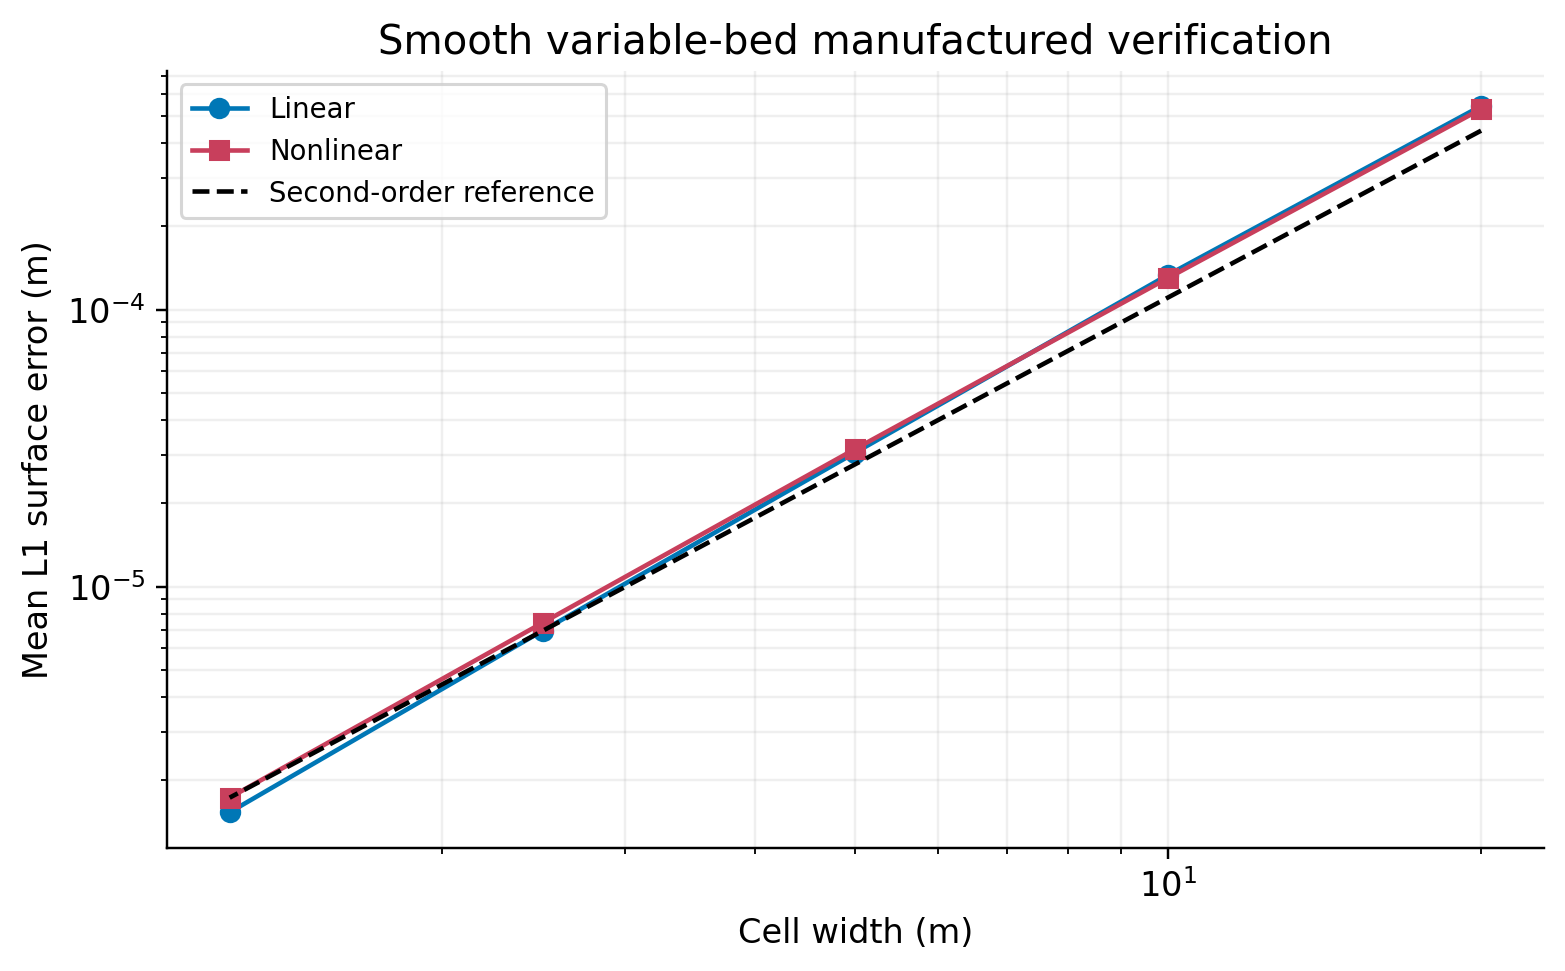
\includegraphics[width=\linewidth]{../figures/final_verification.png}
\caption{Smooth variable-bed manufactured verification. The reference field is
artificially forced; the error decrease verifies implementation, not observations.}
\end{figure}

\section{Experimental design and error interpretation}
\subsection{Matched fields and primary metrics}
Both models receive the same continuous initial surface and velocity; the
nonlinear cell averages are formed from $(h,hu)$, not $(h,Du)$.
At finite resolution $\bar q/\bar h$ need not equal $\bar u$ exactly.
The initial velocity matches a linear right-going wave, so it need not be an
exact nonlinear simple wave. A weak counter-propagating component can therefore
be part of the matched-initial-condition comparison.

The earlier periodic flat-bed sweep measures
$\RMS(\eta_{NL}-\eta_L)/A$, over an entire sine wavelength.
For localized shelf pulses, instead use the domain-normalization-independent
relative norm
\begin{equation}
 E_N=\frac{\norm{\eta_{NL,N}-\eta_{L,N}}}{\norm{\eta_{L,N}}}.
 \label{eq:E}
\end{equation}
These denominators differ; their percentages cannot be directly combined.
If $\mathcal R$ conservatively averages a nested fine mesh onto its coarse mesh,
\begin{equation}
 S_N=\frac{\norm{\mathcal R\eta_{L,N}-\eta_{L,N/2}}
 +\norm{\mathcal R\eta_{NL,N}-\eta_{NL,N/2}}}
 {\norm{\mathcal R\eta_{L,N}}}. \label{eq:S}
\end{equation}
We screen a difference as empirically distinguishable when $E_N/S_N\geq5$.
This is a practical criterion, not a rigorous error bound, confidence interval,
or universal physical-model threshold. Correlated errors may partially cancel.
Peak-height changes between meshes are recorded separately because global
waveform screening does not automatically validate each secondary diagnostic.

\subsection{Flat-bed baseline}
The periodic baseline uses $D=10$ m, $L=1000$ m, $\eta_0=A\sin(2\pi x/L)$,
$u_0=\sqrt{gD}\,\eta_0/D$, and $t=0.2L/\sqrt{gD}$.
For $A/D=0.01,0.05,0.1,0.2$, normalized RMS model differences are
0.625\%, 3.126\%, 6.252\% and 12.505\%, respectively.
The smallest amplitude $10^{-4}$ requires 6400 rather than 3200 cells to pass
the empirical screen. These fixed-time smooth-wave results motivate the shelf
study but do not predict every propagation regime.

\section{Abrupt-step scattering}\label{sec:step}
A Gaussian incident pulse with $A=0.002$ m, $\sigma=120$ m and center
$-1200$ m propagates across a 20-to-5 m depth step at $x=0$.
The domain is $[-4000,4000]$ m and the comparison time is 220 s.
For $f(s)=A\exp[-(s-x_0)^2/(2\sigma^2)]$, the independent linear reference is
\begin{equation}
 \eta(x,t)=\begin{cases}
 f(x-c_lt)+R f(-x-c_lt),&x<0,\\
 T f((c_l/c_r)x-c_lt),&x>0,
 \end{cases}
\end{equation}
where $R=(c_l-c_r)/(c_l+c_r)=1/3$ and $T=2c_l/(c_l+c_r)=4/3$.
Surface and discharge continuity also imply
$R^2+(c_r/c_l)T^2=1$.

\begin{table}[htbp]\centering\small
\begin{tabular}{lrrr}\toprule
Model & $R$ & $T$ & Relative $L^2$ (\%) \\
\midrule
Linear & 0.33273 & 1.32655 & 0.368 \\
Nonlinear, junction & 0.33271 & 1.32630 & 0.792 \\
Nonlinear, HR control & 0.42785 & 1.13631 & 16.448 \\
\bottomrule\end{tabular}
\caption{Step results on 4000 cells. Exact linear coefficients: $R=1/3$, $T=4/3$.}\end{table}

The finest linear error relative to this exact waveform is approximately
0.368\%. The restricted stationary coupling's nonlinear difference is about
0.792\%; it includes finite-amplitude model difference as well as numerical
error, and is not a pure nonlinear numerical-error estimate.

The retained hydrostatic-only control has a 16.45\% waveform discrepancy at
4000 cells and $R\simeq0.428$, despite excellent static and mass checks.
Its failure is reported rather than suppressed. The result establishes a
limitation of this implemented abrupt-step treatment, not a theorem that every
hydrostatic-reconstruction method must have the same error. This experiment
explains why the subcritical coupling is explicit and why smooth-bed tests are
insufficient certification for discontinuous-bed dynamics.
\begin{figure}[htbp]\centering
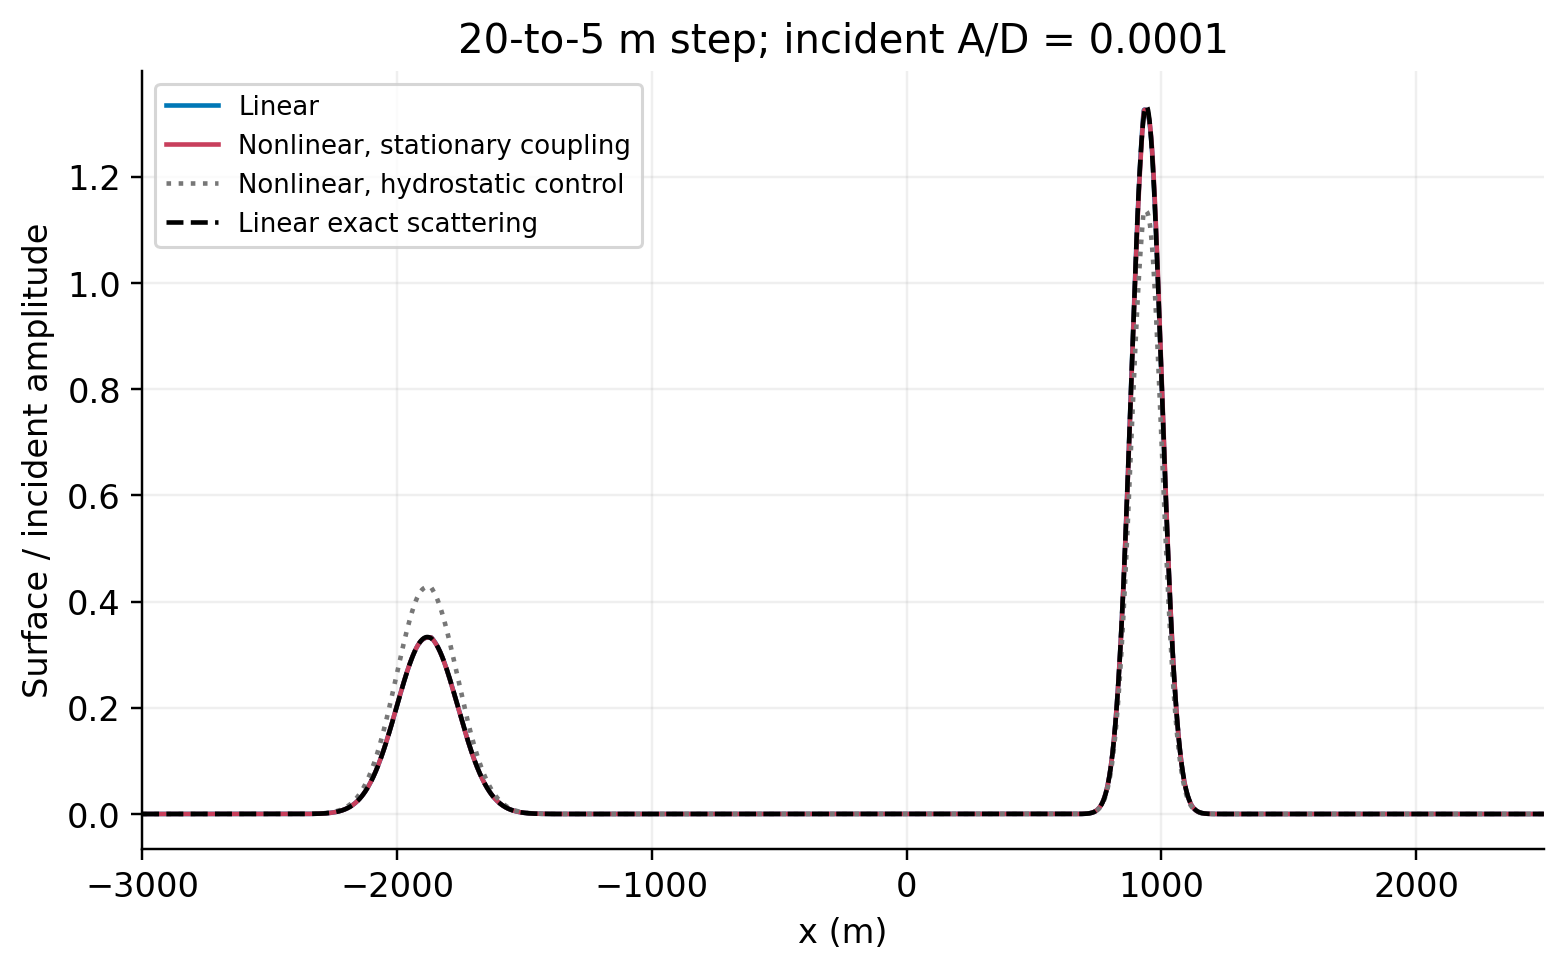
\includegraphics[width=\linewidth]{../figures/final_step_waveform.png}
\caption{Low-amplitude step scattering. The hydrostatic-only control differs
persistently; the subcritical junction coupling recovers the expected small-wave
limit. The nonlinear curves are compared with a linear reference, not an exact
finite-amplitude solution.}
\end{figure}

\section{Smooth-shelf parameter study}
\subsection{Setup}
The domain is $[-8000,8000]$ m. The deep depth is 20 m; shallow/deep ratios
are 0.5 and 0.25. For transition length $\ell\in\{200,800,2400\}$ m, define
$s=\operatorname{clip}(x/\ell+1/2,0,1)$ and
\begin{equation}
 D(x)=D_d+(D_s-D_d)\,[10s^3-15s^4+6s^5].
\end{equation}
The $C^2$ transition joins flat plateaus. The initial Gaussian has center
$-2000$ m and $\sigma=150$ m, with $A/D_d\in\{0.001,0.01,0.05\}$.
The initial tail at the widest transition's start is at most approximately
$6.7\times10^{-7}$ of the pulse peak. Each of the 18 physical cases uses
1000, 2000 and 4000 cells at a final time of 450 s (108 solver runs).
At this time, the principal transmitted pulse is beyond the transition and
its principal reflected component is on the deep plateau.

Transmitted peaks are measured only for $x>\ell/2+3\sigma$; reflected peaks
for $x<-\ell/2-3\sigma$. This spatial separation avoids naming a still-incoming
peak as a reflection. Positive Gaussian tails and distributed reflection remain
limitations of simple peak-based coefficients.

\subsection{Results and the resolution screen}
\begin{table}[htbp]\centering\small
\begin{tabular}{lrrrrr}\toprule
$D_s/D_d$ & $\ell$ (m) & $A/D_d$ & $100E$ & $100S$ & Screen \\
\midrule
0.50 & 200 & 0.001 & 5.02 & 4.12 & Unresolved \\
0.50 & 200 & 0.010 & 46.01 & 7.26 & Pass \\
0.50 & 200 & 0.050 & 96.61 & 6.19 & Pass \\
0.50 & 800 & 0.001 & 5.04 & 4.05 & Unresolved \\
0.50 & 800 & 0.010 & 46.22 & 7.23 & Pass \\
0.50 & 800 & 0.050 & 97.16 & 6.20 & Pass \\
0.50 & 2400 & 0.001 & 4.93 & 3.89 & Unresolved \\
0.50 & 2400 & 0.010 & 45.47 & 7.03 & Pass \\
0.50 & 2400 & 0.050 & 97.02 & 6.08 & Pass \\
0.25 & 200 & 0.001 & 10.05 & 6.50 & Unresolved \\
0.25 & 200 & 0.010 & 71.87 & 10.04 & Pass \\
0.25 & 200 & 0.050 & 101.93 & 6.06 & Pass \\
0.25 & 800 & 0.001 & 10.26 & 6.44 & Unresolved \\
0.25 & 800 & 0.010 & 73.63 & 10.23 & Pass \\
0.25 & 800 & 0.050 & 104.24 & 6.14 & Pass \\
0.25 & 2400 & 0.001 & 9.53 & 6.00 & Unresolved \\
0.25 & 2400 & 0.010 & 71.45 & 10.23 & Pass \\
0.25 & 2400 & 0.050 & 104.51 & 6.16 & Pass \\
\bottomrule\end{tabular}
\caption{Standard-grid shelf study at 4000 cells. $E$ and $S$ have the denominators in equations (\ref{eq:E}) and (\ref{eq:S}); their percentages are not percentages of incident amplitude.}\end{table}

At the standard finest mesh, \ShelfPass\ of 18 cases pass \eqref{eq:S}'s
fivefold screen. The six weak cases require more care: their computed
model differences are of similar scale to accumulated discretization changes.
The reported percentages for failed rows remain exploratory and must not be
read as established physical-model discrepancies.

Two weak, slowly varying cases ($\ell=2400$ m, $\epsilon=0.001$) receive
focused 8000- and 16000-cell follow-up after that initial screen. This selection
is explicitly exploratory rather than pre-registered. Results are
\begin{table}[htbp]\centering\small
\begin{tabular}{lrrrr}\toprule
$D_s/D_d$ & Cells & $100E$ & $100S$ & $E/S$ \\
\midrule
0.50 & 4000 & 4.930 & -- & -- \\
0.50 & 8000 & 4.938 & 1.159 & 4.26 \\
0.50 & 16000 & 4.938 & 0.337 & 14.64 \\
0.25 & 4000 & 9.535 & -- & -- \\
0.25 & 8000 & 9.582 & 1.744 & 5.50 \\
0.25 & 16000 & 9.589 & 0.502 & 19.10 \\
\bottomrule\end{tabular}
\caption{Exploratory focused refinement at $\ell=2400$ m and $A/D_d=0.001$. The two finest rows pass the fivefold screen; the other four weak physical cases have not received this follow-up.}\end{table}


Finite amplitude produces phase changes and steepening over the relatively long
propagation time. For the largest incident amplitude, fronts can become
bore-like; near-second-order smooth-reference results do not apply at those
fronts. No dispersive breaking criterion or calibrated physical dissipation is
included. An $E$ above 100\% is possible for the relative norm \eqref{eq:E}
when two localized packets differ strongly in phase or shape; it does not mean
100\% local height error at every point.
\begin{figure}[htbp]\centering
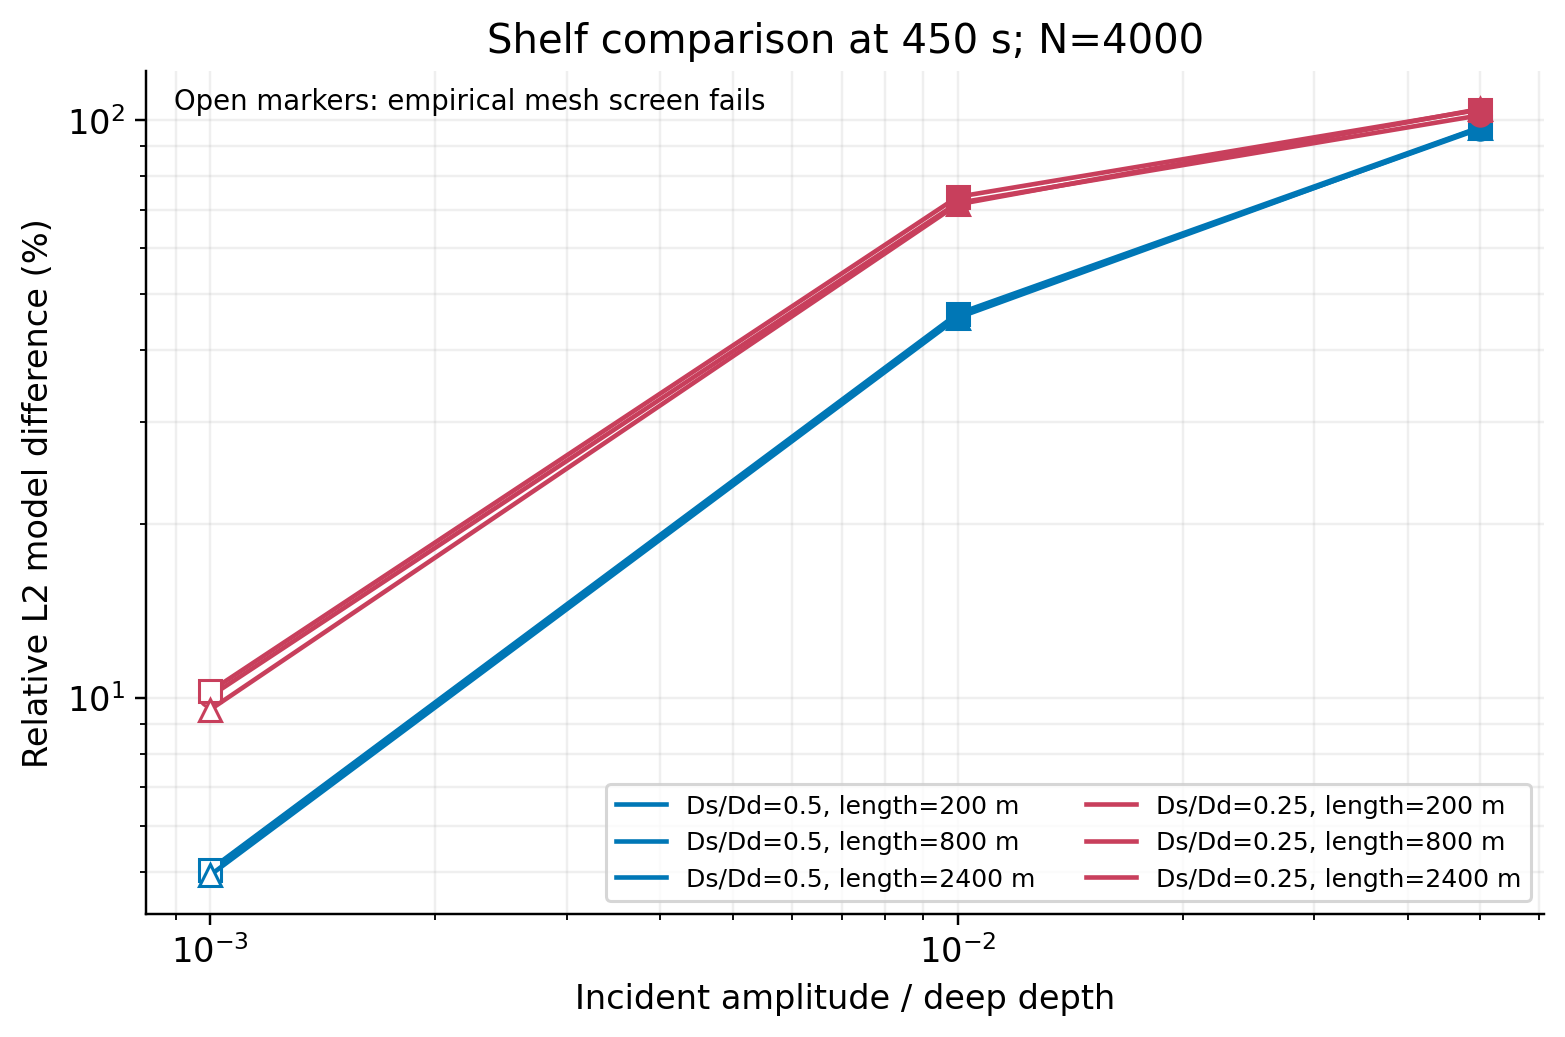
\includegraphics[width=\linewidth]{../figures/final_shelf_difference.png}
\caption{Shelf model differences. Filled symbols pass the empirical fivefold
mesh screen at 4000 cells; open symbols fail it. Focused finer checks are
reported separately. Lines connect sampled cases, not fitted scaling laws.}
\end{figure}

\subsection{Shoaling and reflection}
At 4000 cells and weak amplitude, the linear transmitted peak increases as the
transition becomes more gradual. For shallow/deep ratio 0.5 it is approximately
1.165, 1.174 and 1.179 times the incident amplitude; for ratio 0.25 it is
1.337, 1.376 and 1.392. Green references are 1.189 and 1.414, respectively.
The separate fine-mesh check refines the longest-transition peak estimates.
The standard-grid peak changes and finite transition/reflection prevent treating
these comparisons as an exact verification of Green's law.
\begin{figure}[htbp]\centering
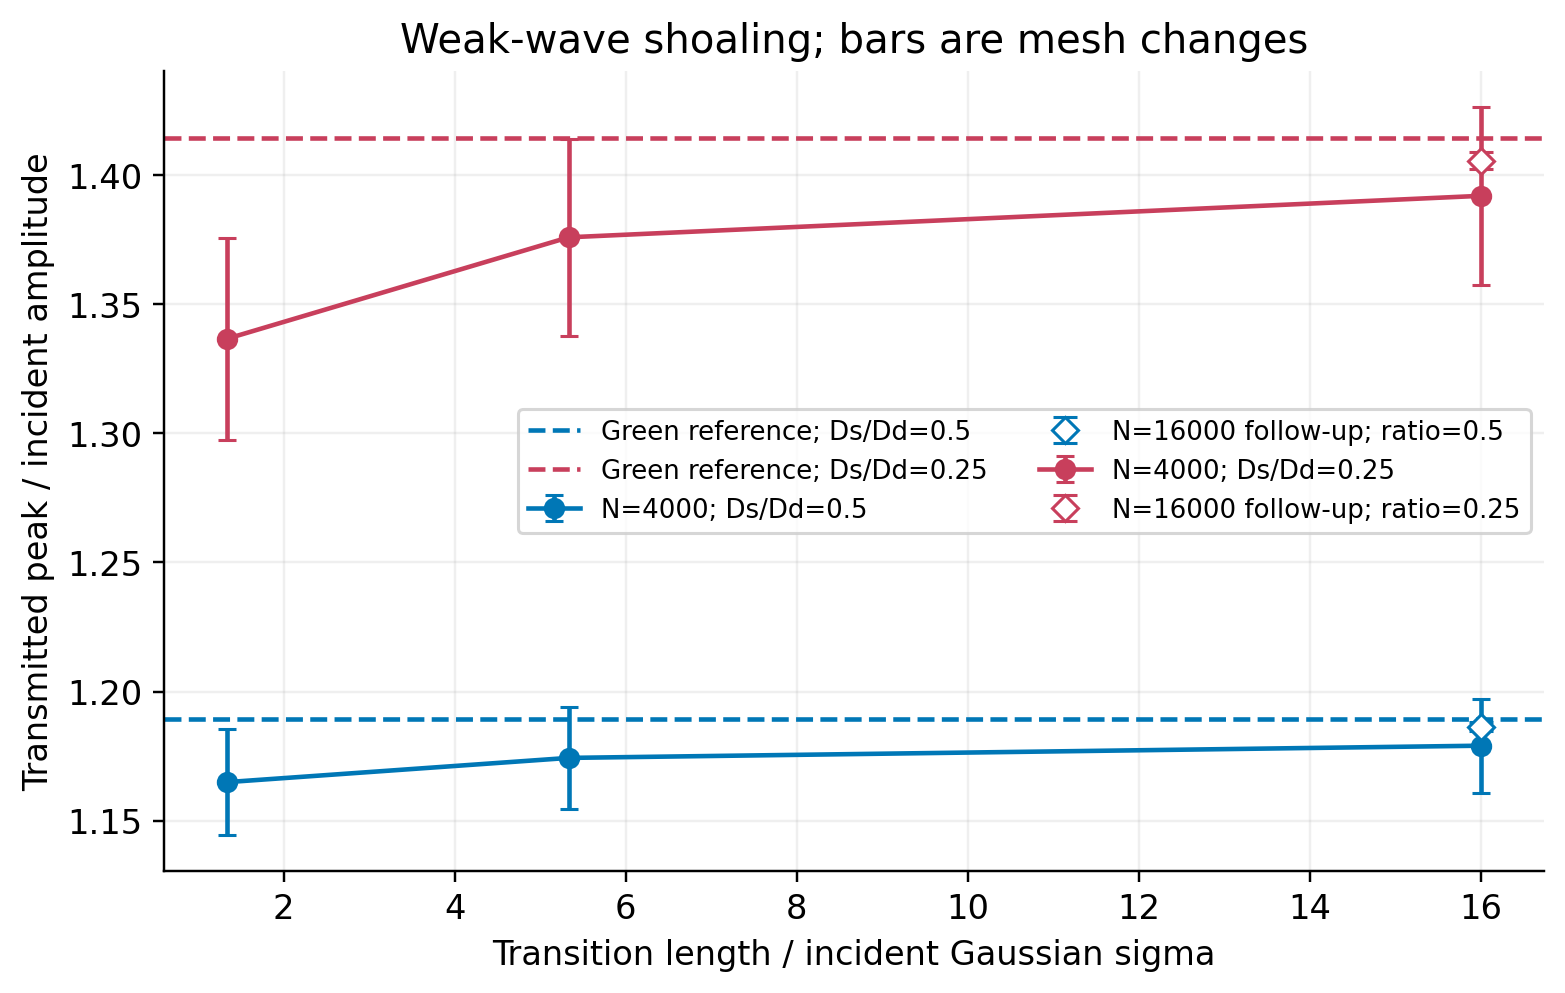
\includegraphics[width=\linewidth]{../figures/final_shoaling.png}
\caption{Weak-wave transmitted peaks and slow-variation references. Error bars
show last-two-mesh changes, not confidence intervals. The fine-grid markers
apply only to the selected longest-transition follow-up cases.}
\end{figure}

\section{Conditional laboratory comparison}\label{sec:lab}
\subsection{Source, geometry and metadata decisions}
The NOAA-hosted USACE composite-beach archive provides 600 rows for Case A,
with original times 265.05--295.00 s sampled every 0.05 s and elevations in
metres \cite{noaa}. The archive identifies an incident gauge at 12.64 m
and downstream gauges at 15.04, 17.22, 19.40, 20.86, 22.33 and 22.80 m,
all measured from the wavemaker. Its reported actual $H/d$ is 0.039.

The webpage instead lists Case A's incident coordinate as 12.22 m and a slightly
different amplitude ratio. We choose the archive's internally associated records
and coordinates, not a mixture of both sources. This unresolved disagreement
is part of the uncertainty of the conditional comparison.
The NOAA figure uses a shoreline/wall-origin coordinate. Converting its
junctions using the 23.22 m wall position gives wavemaker-origin junctions
15.039, 19.399 and 22.329 m, with slopes 1:53, 1:150 and 1:13.
The still-water depth is constructed as
\begin{align}
 D(x)=0.218&-\frac{\operatorname{clip}(x-15.039,0,4.360)}{53}\\
 &-\frac{\operatorname{clip}(x-19.399,0,2.930)}{150}
 -\frac{\max(x-22.329,0)}{13}.
\end{align}
Its wall depth is approximately 0.04766 m, consistent with a fully wet
bounded water-level calculation. Recorded gauge depths have small rounding
and page/archive differences; no fitted geometry adjustment is applied.

\subsection{Preprocessing and withheld comparison}
The first 20 samples of each gauge are averaged and removed as a fixed
pre-arrival baseline. No detrending fit, time translation, amplitude scaling,
filtering fit or parameter calibration follows. Gauge G4 supplies a linearly
interpolated incoming surface signal. The model begins at rest at the original
265.05 s record time and stops at 283 s, giving \LabSamples\ comparison samples.
The upstream boundary is not independently predicted. Six downstream traces
are withheld from the propagation calculation and used for comparison.

The selected window includes the incident downstream response and wall
reflection but ends before the estimated \emph{peak} wall reflection returns
to G4. Pulse tails and possible early outgoing components remain a limitation.
Only water levels are measured; the incident velocity/characteristic is inferred
from the chosen model. These assumptions prevent interpreting the experiment
as independent tsunami-source reconstruction or complete official benchmark
certification.

\subsection{Results}
For each gauge, RMSE is normalized by the maximum absolute baseline-corrected
observed elevation within the specified window, rather than by an optimized
scale. Meshes contain 400, 800 and 1600 cells. The finest results are
\begin{table}[htbp]\centering\small
\begin{tabular}{lrrrrr}\toprule
Gauge & Obs. peak (mm) & L RMSE (\%) & NL RMSE (\%) & L mesh (\%) & NL mesh (\%) \\
\midrule
G5 & 9.14 & 4.06 & 3.96 & 0.12 & 0.12 \\
G6 & 8.87 & 5.37 & 5.57 & 0.21 & 0.17 \\
G7 & 10.06 & 6.52 & 9.45 & 0.22 & 0.52 \\
G8 & 10.06 & 9.34 & 10.17 & 0.31 & 0.40 \\
G9 & 11.28 & 9.64 & 9.38 & 0.29 & 0.42 \\
G10 & 16.15 & 4.97 & 8.08 & 0.22 & 0.47 \\
\bottomrule\end{tabular}
\caption{Conditional Case A comparison at 1600 cells. RMSE and last-two-grid RMS change are normalized by each observed absolute peak in the fixed window. These are not confidence intervals.}\end{table}

The linear normalized RMS range is \LabLinearRange\, and the nonlinear range
is \LabNonlinearRange. Mesh changes are appreciably smaller than the main
observation discrepancies for most traces; they do not account for metadata,
input-decomposition, dispersion, friction or measurement uncertainty.
Nonlinearity is not uniformly beneficial. At gauges with incident and reflected
peaks, the global maximum can switch branches, so a reported maximum-time
shift is not automatically an arrival-time error.
\begin{figure}[p]\centering
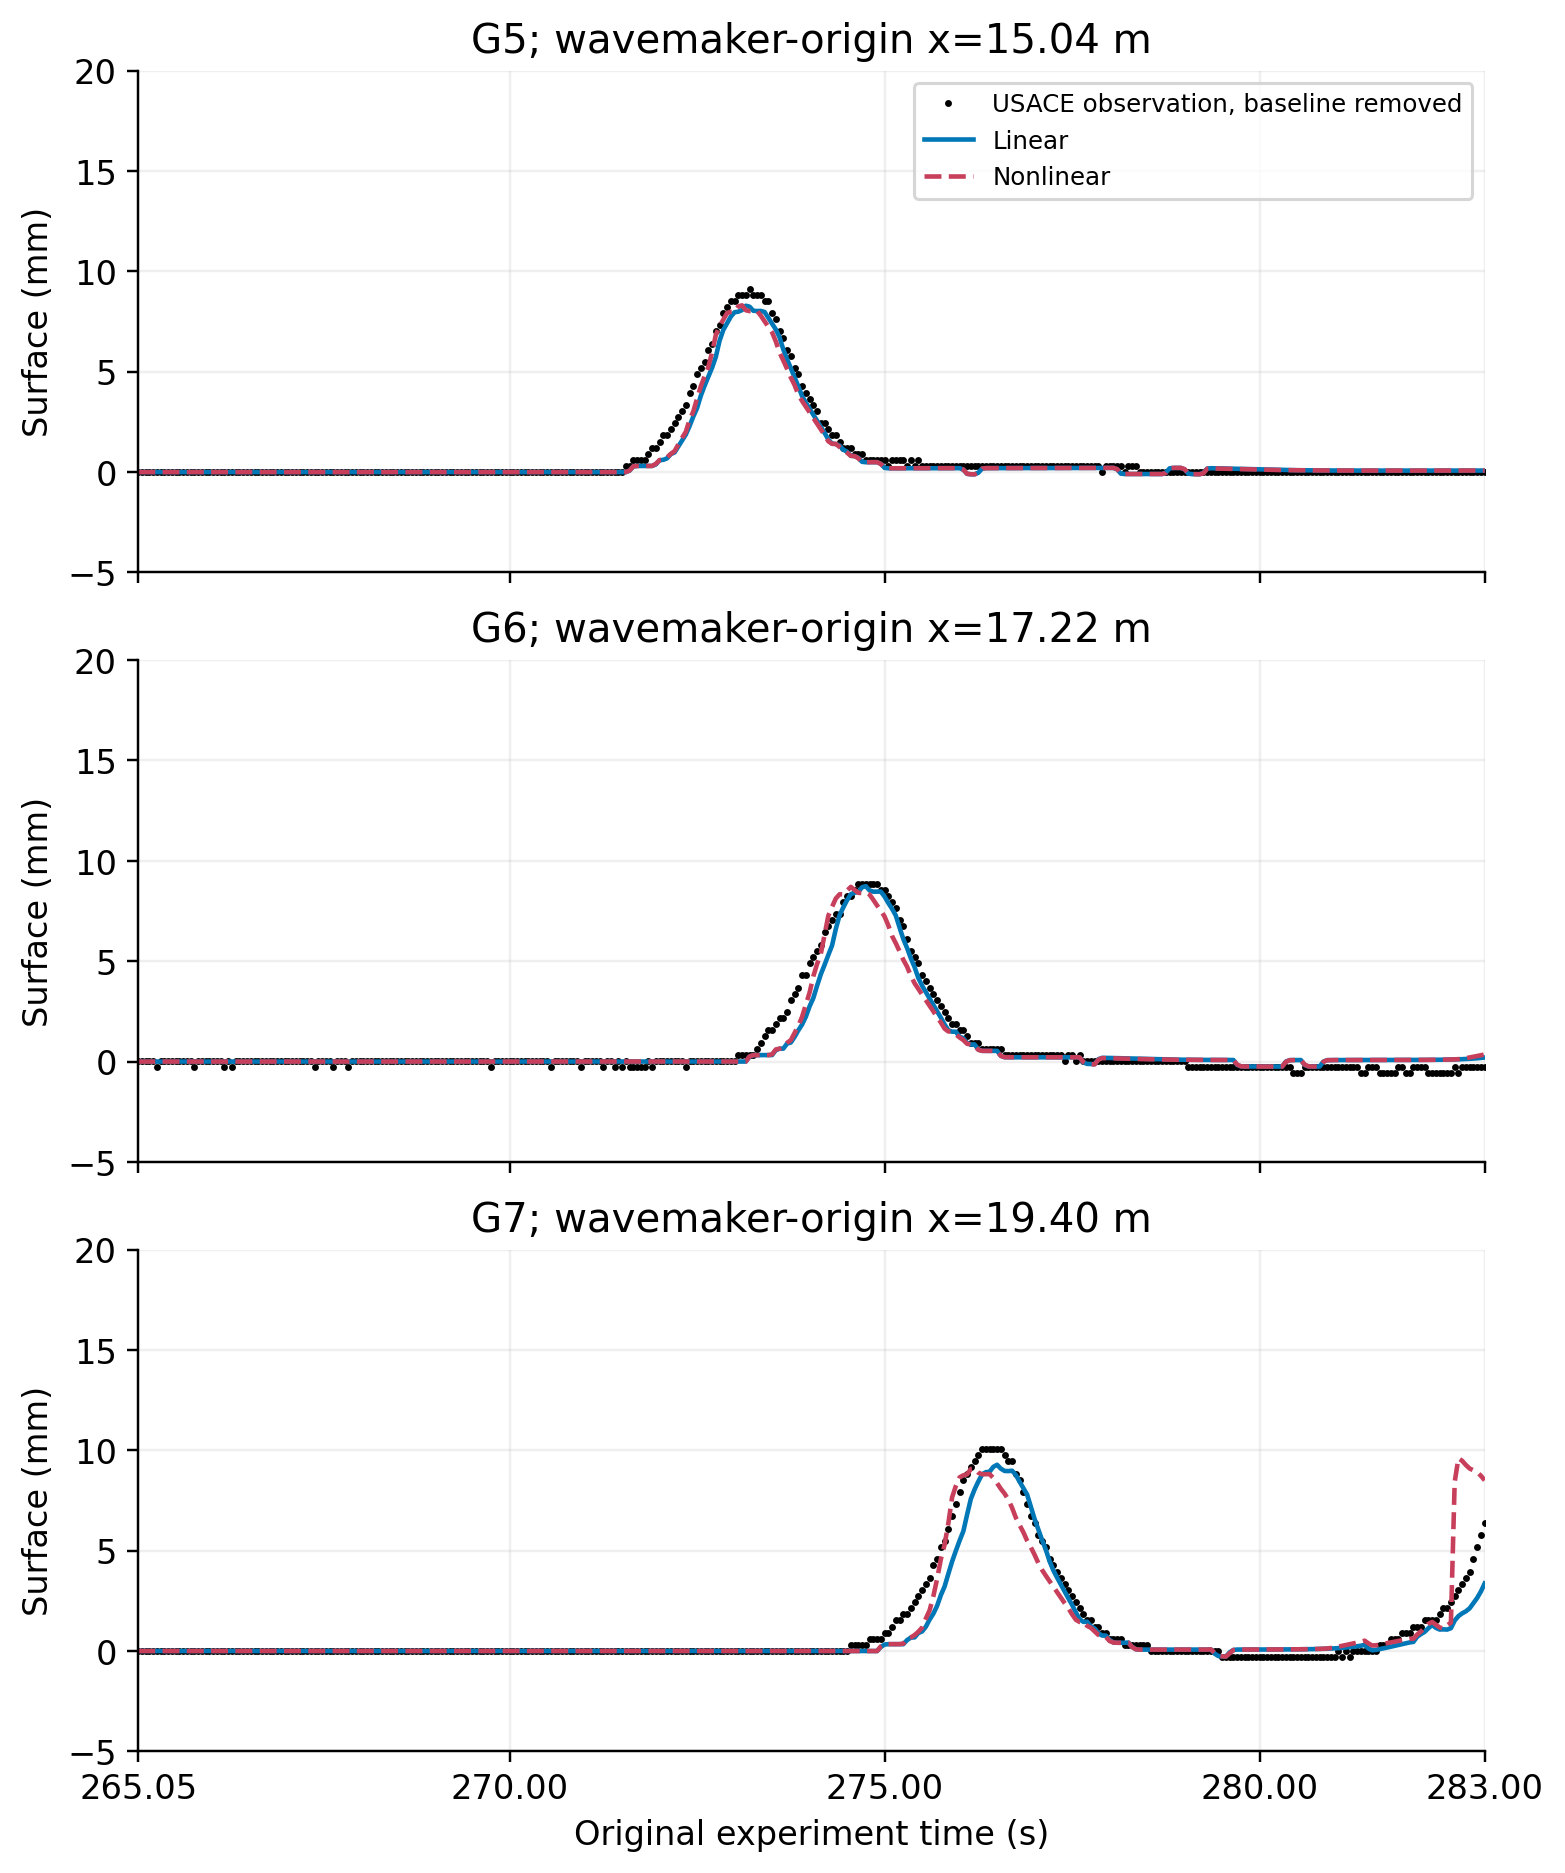
\includegraphics[width=.96\linewidth]{../figures/final_lab_upstream.png}
\caption{Case A downstream gauges G5--G7. The upstream G4 record is the input;
these traces are predictions. Original experiment time is retained.}
\end{figure}
\begin{figure}[p]\centering
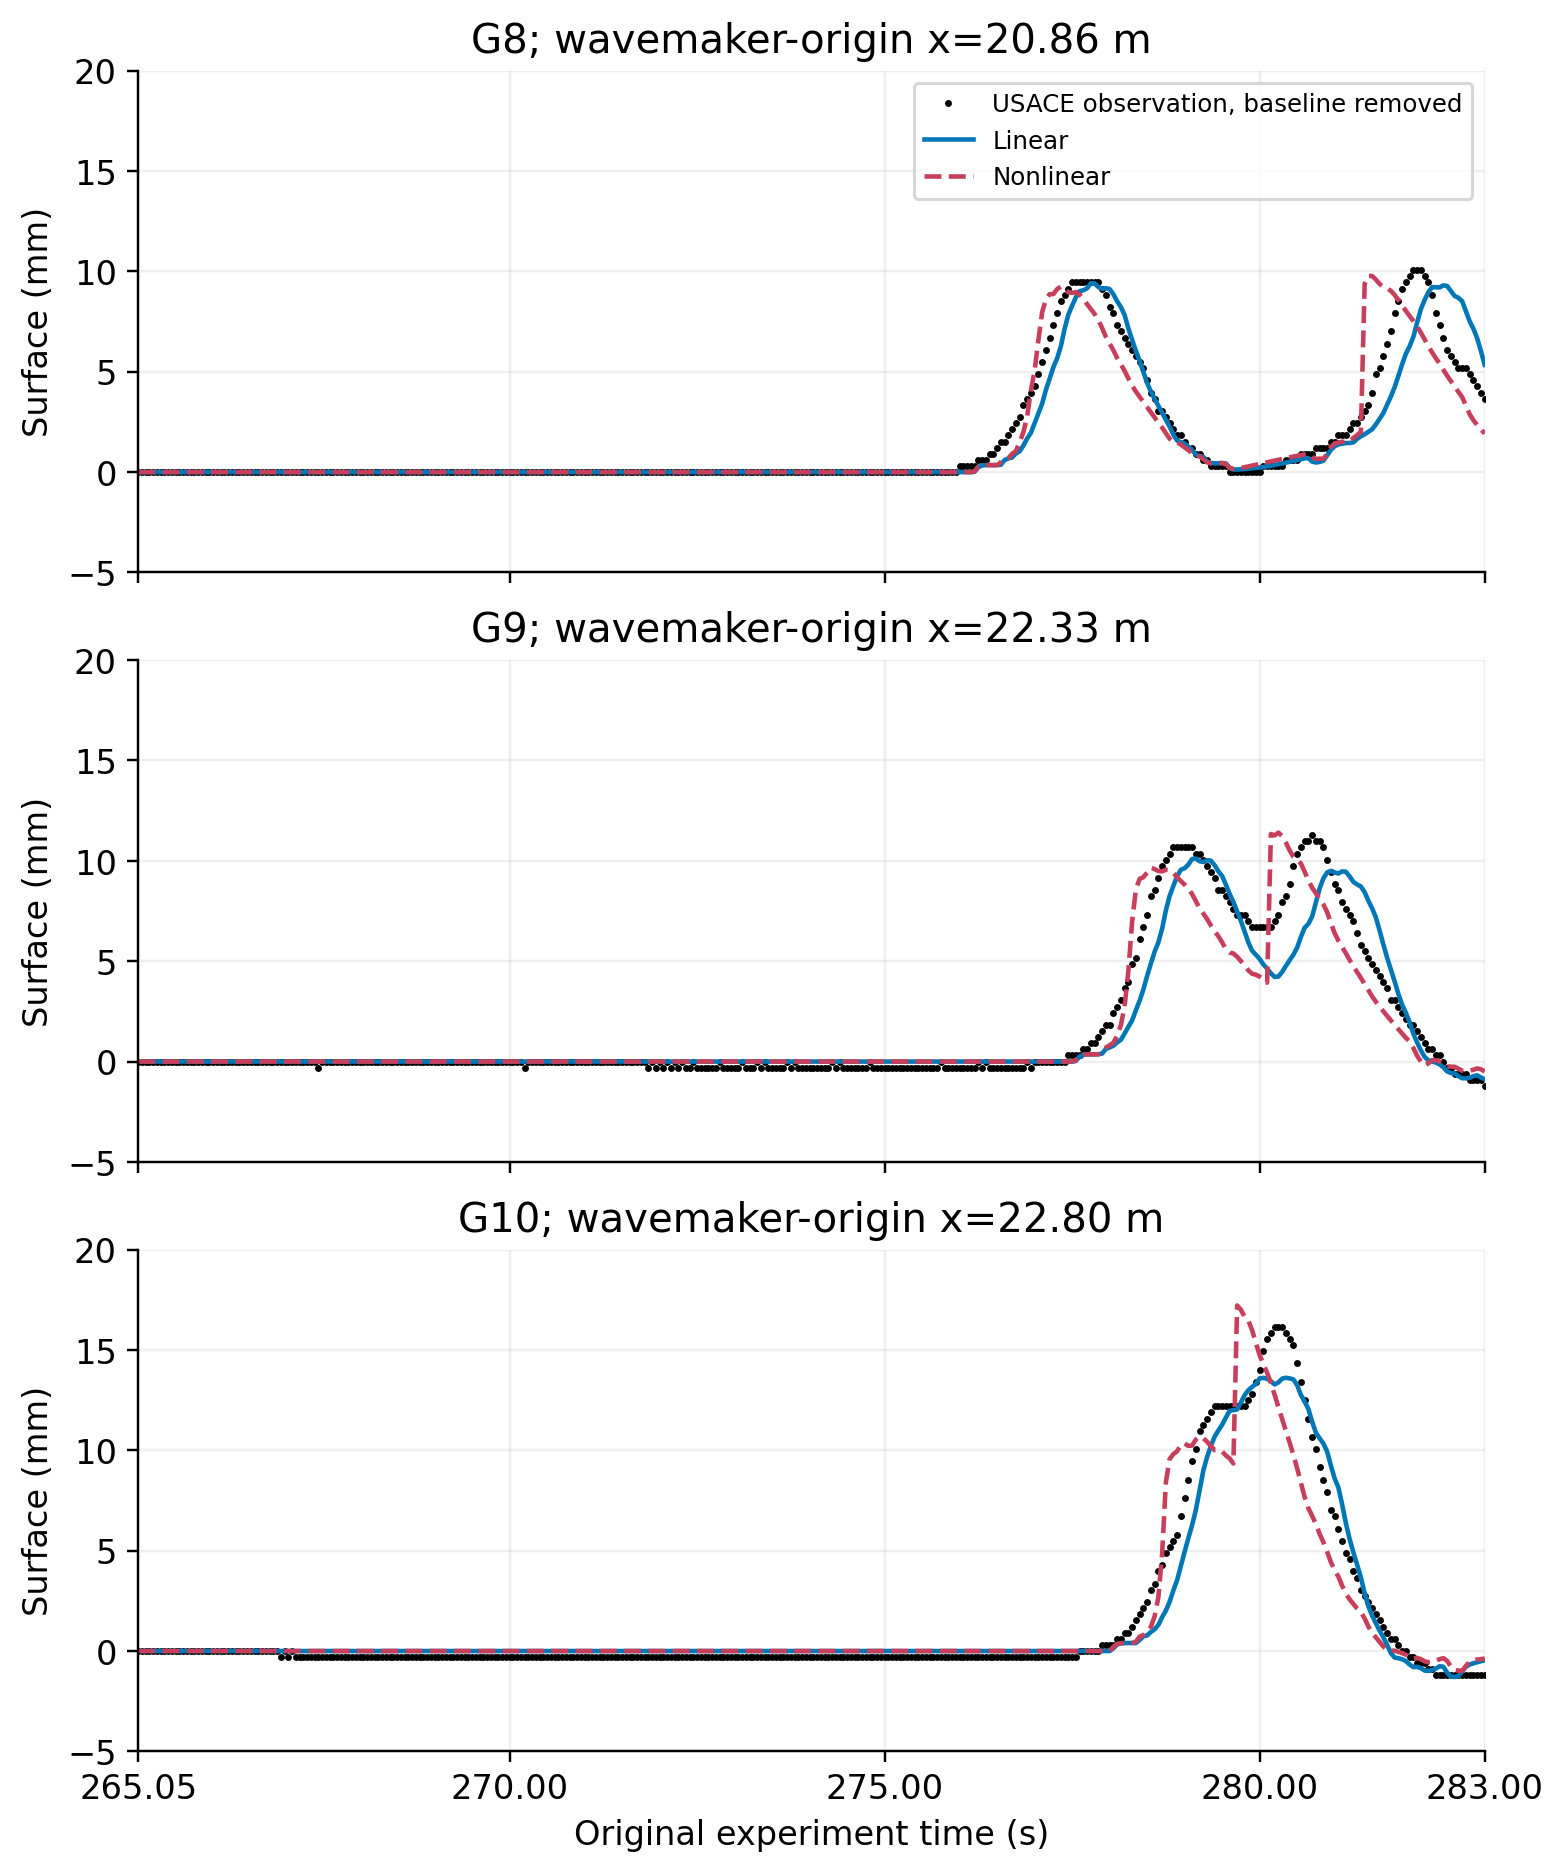
\includegraphics[width=.96\linewidth]{../figures/final_lab_downstream.png}
\caption{Case A gauges G8--G10, including wall-reflected contributions. No fitted
time shift is used. Discrepancies and changing dominant peaks are retained.}
\end{figure}

\section{Limitations and conclusions}
This project supports the following conclusions within its tested scope:
\begin{enumerate}
\item Equilibrium-preserving reconstruction and source accounting are necessary
checks, but do not certify all dynamic wave behavior. The abrupt-step control
provides a concrete counterexample in the implemented method.
\item Under weak subcritical step scattering, explicit discharge/head matching
recovers the expected linear limit substantially better than the retained control.
It remains a restricted junction model.
\item In smooth-shelf runs, incident amplitude, local depth and propagation time
jointly affect linear/nonlinear differences. The 18-case screen prevents
unresolved weak-wave differences from being promoted to physical conclusions.
\item More gradual transitions give weak-wave transmitted peaks closer to the
slow-variation reference in this sample, subject to mesh sensitivity and reflection.
\item A conditional laboratory comparison is feasible without fitting downstream
traces, but additional nonlinearity does not consistently reduce observational
error. The selected setup and metadata choice bound the claim.
\end{enumerate}
No universal $A/D$ validity cutoff, real-event forecast accuracy, calibrated
breaking/dissipation, inundation map or shoreline run-up result follows from this
study. The shelf family is idealized and finite; statistical uncertainty intervals
are not estimated. The grid screen is empirical. Shock-local accuracy, long-time
accumulation and incoming-boundary assumptions can dominate particular metrics.

A journal submission would require a sharper novel contribution, broader
literature comparison and further independent validation. The present deliverable
is a completed computational project report with research-style derivation,
methods, results, limitations and reproducibility. Extensions include dispersive
models, wet/dry treatment, uncertainty-aware incident decomposition and comparison
with an independently configured mature code, none of which is claimed here.

\appendix
\section{Reproducibility and artifact map}
The archive includes original Python code, 35 standard-library unit tests,
configuration files, experiment scripts, result tables, scientific figures,
animations, a runnable companion notebook, an offline interactive viewer,
this report's LaTeX source and the compiled PDF. Third-party raw observations
are not redistributed under the software's MIT license.
\begin{verbatim}
python -m pip install -r requirements.txt
python scripts/run_verification.py
python scripts/run_final_studies.py
python scripts/run_weak_refinement.py --ratio 0.5
python scripts/run_weak_refinement.py --ratio 0.25
python scripts/build_final_figures.py
python scripts/build_visualizations.py
\end{verbatim}
A unified runner also reproduces the earlier V0.2/V0.3 numerical foundations.
The main scientific pipeline does not require Jupyter or a display. The
laboratory section downloads and checksum-verifies the pinned NOAA archive
when its private raw cache is absent. Offline users can inspect all supplied
predictions and figures, or run the synthetic sections without the lab download.

CSV files expose every standard-grid case and mesh; NPZ files hold numerical
profiles and laboratory predictions. The source-data checksum and metadata
conflicts are recorded in \texttt{data/noaa\_provenance.json} and the data audit.
Run records capture dependency versions and configurations; release checksums
identify the delivered files. Reference figures and tables are generated directly
from result files rather than manually entered. Historical releases are retained
and clearly labeled, not retroactively assigned the V1.0 tests or algorithms.

\section{Software and authorship statement}
The software is original implementation of established equations and numerical
methods. No third-party solver source is copied, and the report does not claim
those methods as inventions. AI assistance was used for code drafting,
documentation and analysis organization. The provided source, executed checks and result files support independent review
and reproduction. This statement records the assistance used in preparing the
computational project.

\begin{thebibliography}{9}
\bibitem{audusse} E. Audusse, F. Bouchut, M.-O. Bristeau, R. Klein and B. Perthame
(2004). A Fast and Stable Well-Balanced Scheme with Hydrostatic Reconstruction
for Shallow Water Flows. \emph{SIAM J. Sci. Comput.} 25(6), 2050--2065.
\href{https://doi.org/10.1137/S1064827503431090}{doi:10.1137/S1064827503431090}.
\bibitem{ssp} S. Gottlieb, C.-W. Shu and E. Tadmor (2001). Strong
Stability-Preserving High-Order Time Discretization Methods.
\emph{SIAM Review} 43(1), 89--112.
\href{https://doi.org/10.1137/S003614450036757X}{doi:10.1137/S003614450036757X}.
\bibitem{riemann} D. I. Ketcheson, R. J. LeVeque and M. J. del Razo.
\emph{Riemann Problems and Jupyter Solutions}, author-maintained online
shallow-water chapter. \url{https://www.clawpack.org/riemann_book/html/Shallow_water.html}.
\bibitem{lefloch} P. G. LeFloch and M.-D. Thanh (2007).
The Riemann problem for the shallow water equations with discontinuous topography.
\href{https://arxiv.org/abs/0712.3778}{arXiv:0712.3778}.
\bibitem{delestre} O. Delestre, S. Cordier, F. Darboux and F. James (2012).
A limitation of the hydrostatic reconstruction technique for Shallow Water equations.
\href{https://arxiv.org/abs/1206.4986}{arXiv:1206.4986}.
\bibitem{green} G. Green. On the Motion of Waves in a variable canal of small
depth and width. In \emph{Mathematical Papers of the Late George Green},
N. M. Ferrers, ed., pp. 223--230; Cambridge digital edition.
\href{https://doi.org/10.1017/CBO9781107325074.007}{doi:10.1017/CBO9781107325074.007}.
\bibitem{noaa} NOAA Center for Tsunami Research.
Solitary Wave on a Composite Beach; NOAA-hosted USACE laboratory data.
\url{https://nctr.pmel.noaa.gov/benchmark/Solitary_wave/}.
Archive: \texttt{tsunami3\_runup.zip}; accessed October 2, 2026.
\bibitem{synolakis} C. E. Synolakis (1987). The runup of solitary waves.
\emph{Journal of Fluid Mechanics} 185, 523--545.
Canonical benchmark context: \url{https://nctr.pmel.noaa.gov/benchmark/Laboratory/Laboratory_CanonicalBathymetry/index.html}.
\end{thebibliography}
\end{document}
